% Skeleton LaTeX report for the RL project
\documentclass[11pt,a4paper]{article}

\usepackage[T1]{fontenc}
\usepackage[utf8]{inputenc}
\usepackage[romanian]{babel}
\usepackage[margin=2.5cm]{geometry}
\usepackage{amsmath, amssymb}
\usepackage{graphicx}
\usepackage{booktabs}
\usepackage{hyperref}
\usepackage{csquotes}
\usepackage{tikz}
\usetikzlibrary{arrows.meta, positioning}

% Include diagram macros
% Diagrams for RL project (compile with LaTeX)

\usepackage{tikz}
\usetikzlibrary{arrows.meta, positioning}

% RL loop diagram
\newcommand{\RLLoopDiagram}{%
  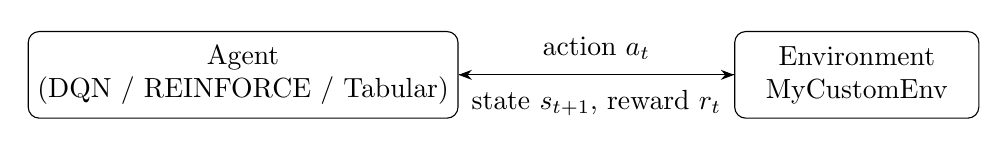
\begin{tikzpicture}[
    node distance=3.5cm,
    >=Stealth,
    box/.style={rectangle, draw, rounded corners, minimum width=3.1cm, minimum height=1.1cm, align=center}
  ]
    \node[box] (agent) {Agent\\(DQN / REINFORCE / Tabular)};
    \node[box, right=of agent] (env) {Environment\\MyCustomEnv};

    % Slightly lifted/lowered labels to avoid overlap with boxes
    \draw[->] (agent) -- node[above,yshift=2pt]{action $a_t$} (env);
    \draw[->] (env)  -- node[below,yshift=-2pt]{state $s_{t+1}$, reward $r_t$} (agent);
  \end{tikzpicture}%
}

% DQN network architecture diagram (high level)
\newcommand{\DQNArchitectureDiagram}{%
  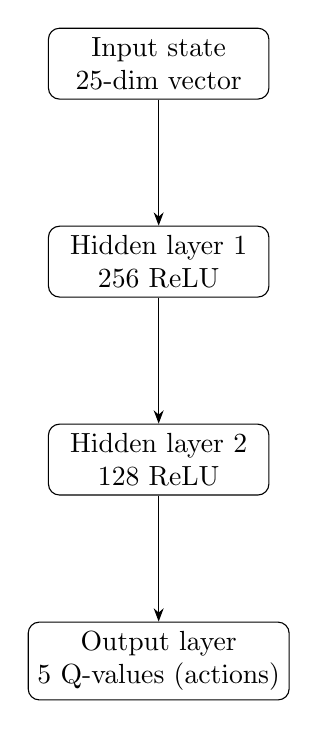
\begin{tikzpicture}[
    node distance=1.6cm,
    >=Stealth,
    layer/.style={rectangle, draw, rounded corners, minimum width=2.8cm, minimum height=0.9cm, align=center}
  ]
    \node[layer] (input) {Input state\\25-dim vector};
    \node[layer, below=of input] (h1) {Hidden layer 1\\256 ReLU};
    \node[layer, below=of h1] (h2) {Hidden layer 2\\128 ReLU};
    \node[layer, below=of h2] (output) {Output layer\\5 Q-values (actions)};

    \draw[->] (input) -- (h1);
    \draw[->] (h1) -- (h2);
    \draw[->] (h2) -- (output);
  \end{tikzpicture}%
}

% Agent comparison conceptual diagram
\newcommand{\AgentComparisonDiagram}{%
  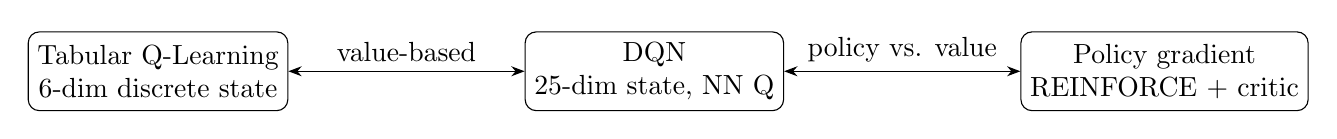
\begin{tikzpicture}[
    node distance=3.0cm,
    >=Stealth,
    box/.style={rectangle, draw, rounded corners, minimum width=2.8cm, minimum height=1cm, align=center}
  ]
    \node[box] (tabular) {Tabular Q-Learning\\6-dim discrete state};
    \node[box, right=of tabular] (dqn) {DQN\\25-dim state, NN Q};
    \node[box, right=of dqn] (reinforce) {Policy gradient\\REINFORCE + critic};

    \draw[<->] (tabular) -- node[above]{value-based} (dqn);
    \draw[<->] (dqn) -- node[above]{policy vs. value} (reinforce);
  \end{tikzpicture}%
}


\title{Reinforcement Learning pentru conducere autonomă într-un mediu personalizat ``Highway''}
\author{Echipa Juno \\ Corobana Ingrid \\ Moise Irina \\ Prizlopan Iustin \\ Sescu Matei}
\date{Ianuarie 2026}

\begin{document}

\maketitle

\section{Formularea problemei}

Obiectivul proiectului este antrenarea unui agent de control pentru un vehicul \emph{ego} (mașina galbenă)
într-un mediu de trafic. Agentul trebuie să circule pe un drum cu mai multe benzi, să evite
coliziunile cu vehiculele din trafic (mașinile albastre), să rămână pe carosabil și, în același timp,
să mențină o viteză rezonabilă.

Problema este formulată ca o problemă de \textbf{Reinforcement Learning (RL)}, în care agentul învață
o politică (\emph{policy}) exclusiv pe baza recompensei primite de la mediu.

\subsection{Stare, acțiune, recompensă}

Modelăm problema în termeni de \emph{stare}, \emph{acțiune} și \emph{recompensă} astfel:
\begin{itemize}
  \item \textbf{Stare (observație):} observația de bază a mediului este de tip \emph{Kinematics}
  (din pachetul \texttt{highway\_env}). După aplicarea \texttt{FlatObsWrapper}, obținem un vector
  continuu de dimensiune \textbf{25}, care conține poziția, viteza și orientarea vehiculului \emph{ego},
  plus informații agregate despre câteva vehicule din proximitate.
  \item \textbf{Acțiune}: mediul original are acțiuni continue (accelerație și direcție). Pentru agenții
  discreți folosim un wrapper \texttt{DiscreteActionWrapper} care definește \textbf{5 acțiuni}:
  \emph{Idle} (0), \emph{Accelerate} (1), \emph{Brake} (2), \emph{Left} (3), \emph{Right} (4).
  \item \textbf{Recompensă}: funcția de recompensă din \texttt{custom\_env.py} combină mai multe
  componente: penalizări puternice pentru \textbf{coliziune} sau \textbf{ieșirea de pe drum} și
  termeni pozitivi pentru \textbf{viteză ridicată} (aliniată cu sensul benzii) și pentru
  	\textbf{menținerea poziției aproape de centrul benzii} (\emph{lane centering}). În acest fel,
  agentul primește feedback la fiecare pas de timp, nu doar la finalul episodului.
\end{itemize}

Diagrama generală agent--mediu este prezentată în Figura~\ref{fig:rl-loop}.
\begin{figure}[h]
  \centering
  \RLLoopDiagram
  \caption{Schema generala agent--mediu folosita in proiect.}
  \label{fig:rl-loop}
\end{figure}

\section{Environment Design}

Mediul este construit pornind de la pachetul \texttt{highway\_env}, însă logica drumului și a
traficului a fost rescrisă în fișierul \texttt{custom\_env.py}.

Drumul este reprezentat ca un graf de benzi (\texttt{RoadNetwork}) și include mai multe secțiuni:
un segment drept de intrare, o zonă de îmbinare (\emph{merge}) cu o bandă laterală, un viraj
circular, porțiuni drepte suplimentare și o ieșire verticală către un nod final \texttt{c0}.
Sunt definite mai multe benzi folosind clasele \texttt{StraightLane} și \texttt{CircularLane},
inclusiv o bandă de intrare laterală pentru vehiculele care se încadrează în trafic.

Vehiculele din trafic sunt de tip \texttt{IDMVehicle} (model de conducere IDM) și sunt plasate
atât pe secțiuni fixe (obstacole poziționate manual), cât și aleator pe drum. Pentru unele
vehicule folosim metoda \texttt{plan\_route\_to} pentru a le forța să urmeze un traseu prin
rețea (de exemplu, de la nodul \texttt{b0} la \texttt{c0}). La fiecare pas de timp,
  	exttt{highway\_env} actualizează automat dinamica tuturor vehiculelor.

Episodul se termină atunci când vehiculul \emph{ego} se ciocnește sau părăsește drumul, iar
trunchierea se produce când timpul depășește \texttt{config["duration"]}. Aceste condiții asigură
episoade finite și un semnal de învățare bine definit pentru toți agenții.

\section{Algoritmi}

În același mediu am antrenat și comparat trei tipuri de agenți:
un agent tabular (Q-Learning), un agent DQN și un agent de tip policy gradient
(REINFORCE cu baseline de valoare).

\subsection{Tabular Q-Learning}

Agentul tabular folosește o reprezentare discretizată a stării, obținută prin wrapper-ul
  exttt{TabularObsWrapper}. Observația continuă este proiectată într-un vector de 6 componente:
poziția \emph{ego} pe o grilă 2D (x, y), un nivel discretizat de combustibil și două variabile
discrete care codifică direcția aproximativă către țintă (dx, dy), împreună cu o componentă binară
simplă de context. Dimensiunile de discretizare sunt $[6, 6, 3, 2, 3, 3]$, rezultând 1944 de stări
posibile.

Pentru fiecare stare discretă se păstrează o valoare $Q(s,a)$ într-un tabel cu 5 acțiuni. Actualizarea
este cea clasică de Q-Learning:
\[
Q(s,a) \leftarrow Q(s,a) + \alpha \bigl(r + \gamma \max\limits_{a'} Q(s', a') - Q(s,a)\bigr),
\]
cu factor de învățare $\alpha = 0{,}05$, factor de discount $\gamma = 0{,}99$ și o strategie
$\varepsilon$-greedy pentru explorare, cu $\varepsilon$ care scade treptat de la 1 la 0.05.

\subsection{Deep Q-Network (DQN)}

Agentul DQN folosește direct vectorul continuu de 25 de dimensiuni ca intrare într-o rețea neuronală
feed-forward. Arhitectura implementată în proiect este:
\begin{itemize}
  \item strat de intrare: vectorul de stare (25 dimensiuni);
  \item două straturi ascunse dense cu 256 și respectiv 128 de neuroni și activare ReLU;
  \item strat de ieșire: 5 neuroni care produc valorile $Q(s,a)$ pentru fiecare acțiune discretă.
\end{itemize}

Rețeaua este antrenată folosind experience replay (buffer de 50\,000 de tranziții) și un
\emph{target network} sincronizat periodic. La fiecare pas, o tranziție $(s,a,r,s',\text{done})$
este adăugată în buffer, iar când există suficiente exemple se eșantionează mini-loturi de mărime 64.
Țintelor de învățare li se aplică fie formula clasică DQN, fie varianta Double DQN (selecție
de acțiune cu \texttt{policy\_net}, evaluare cu \texttt{target\_net}). Funcția de pierdere este
Huber (\texttt{SmoothL1Loss}). Explorarea se face cu o strategie $\varepsilon$-greedy cu
$\varepsilon$ care scade de la 1.0 la 0.01.

Diagrama de arhitectura DQN este prezentata in Figura~\ref{fig:dqn-arch}.
\begin{figure}[h]
  \centering
  \DQNArchitectureDiagram
  \caption{Arhitectura DQN care mapeaza starea la valorile $Q(s,a)$ pentru cele 5 actiuni.}
  \label{fig:dqn-arch}
\end{figure}

\subsection{Policy Gradient (REINFORCE + Baseline)}

Al treilea agent este unul de tip policy-based. Politica $\pi_\theta(a\mid s)$ este
parametrizată de o rețea neuronală (\texttt{PolicyNetwork}) cu un singur strat ascuns de 64
neuroni și ieșire softmax peste cele 5 acțiuni. În plus, am introdus un \emph{value network}
care aproximează funcția de valoare $V_\phi(s)$ și este antrenat împreună cu politica.

Update-ul folosește REINFORCE cu advantage:
\[
\nabla J(\theta) \approx \sum_t \log \pi_\theta(a_t \mid s_t) \cdot A_t, \quad
A_t = G_t - V_\phi(s_t),
\]
unde $G_t$ este returnul Monte Carlo din pasul $t$. Valoarea este antrenată cu eroare pătratică
față de $G_t$, iar pierderea totală este suma dintre pierderea de politică și o componentă de
valoare ponderată. Acest baseline reduce varianța gradientului și îmbunătățește stabilitatea
față de REINFORCE simplu.

\section{Experimente}

Obiectivul experimental a fost compararea celor trei agenți (tabular, DQN și
REINFORCE cu baseline) în exact același mediu și cu același set de acțiuni
discrete. Pentru fiecare agent am definit un script separat de antrenare
(\texttt{train\_tabular.py}, \texttt{train\_dqn.py}, \texttt{train\_reinforce.py}) și am păstrat
aceleași condiții de inițializare ale mediului.

Pentru DQN și agentul tabular am rulat câte 500 de episoade de antrenare,
în timp ce pentru REINFORCE am folosit 1000 de episoade pentru a compensa
varianța mai mare a gradientului de politică. La fiecare episod am înregistrat
recompensa cumulată și am salvat un model „best” pe baza mediei mobile a
ultimelor 20--50 de episoade.

Pentru a vizualiza evoluția antrenării, scriptul \texttt{plot\_results.py} încarcă
fișierele CSV generate de fiecare agent și desenează curbele de recompensă,
împreună cu o versiune netezită. Figura~\ref{fig:training} arată clar viteza de
convergență și nivelul final de performanță pentru fiecare algoritm.

\subsection{Curbe de antrenare}

\begin{figure}[h]
  \centering
  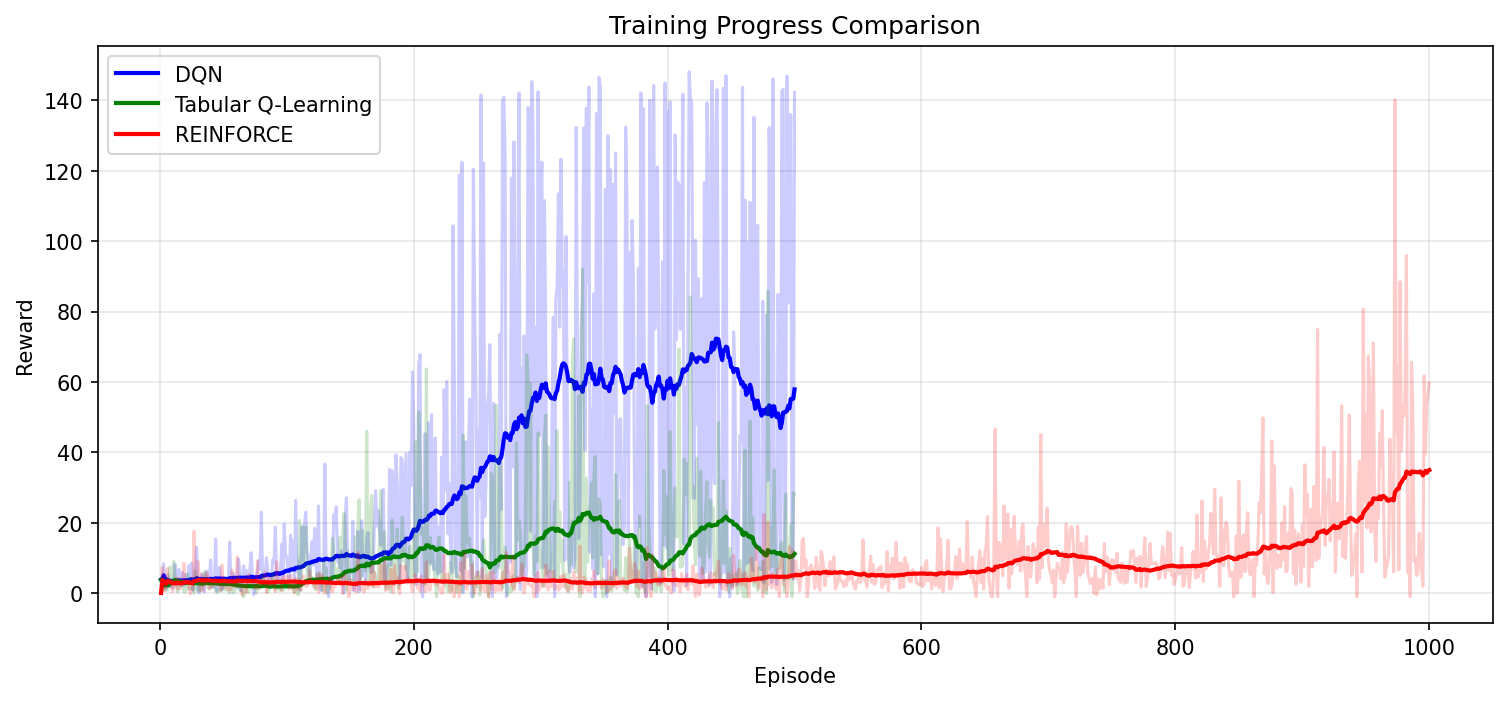
\includegraphics[width=0.9\linewidth]{../results/training_comparison.png}
  \caption{Curbele de recompensă în timpul antrenării pentru toți cei trei agenți.}
  \label{fig:training}
\end{figure}

\subsection{Evaluare și comportament}

Am implementat și scriptul de evaluare \texttt{evaluate\_agents.py}, care
încarcă modelele antrenate și rulează un număr fix de episoade de test pentru
fiecare agent, cu politică pur deterministă (fără explorare, $\varepsilon=0$).
Rezultatele sunt salvate în fișiere CSV și reprezentate grafic într-un barplot
(\texttt{eval\_barplot.png}), care permite compararea directă a recompenselor medii.

Comportamentul calitativ al agenților a fost analizat și prin \texttt{visualize\_actions.py},
care desenează pe hartă pozițiile mașinii \emph{ego}, colorate în funcție de acțiunea aleasă
(accelerare, frânare, schimbare de bandă etc.). Aceste hărți de acțiuni ajută la interpretarea
tiparelor învățate de fiecare algoritm.

\subsection{Hiperparametri și diagrame}

Pentru fiecare agent am ales un set de hiperparametri care echilibrează stabilitatea și viteza de
învățare:
\begin{itemize}
  \item \textbf{Tabular Q-Learning}: $\alpha = 0{,}05$, $\gamma = 0{,}99$, \mbox{$\varepsilon \in [1, 0{,}05]$}
  cu decay; rata de învățare relativ mică evită oscilațiile într-un spațiu de stare discret dar dens,
  iar discount-ul mare pune accent pe recompensele viitoare (traiectorii sigure și lungi).
  \item \textbf{DQN}: rata de învățare $5\cdot 10^{-4}$, $\gamma = 0{,}99$, buffer de 50\,000 tranziții,
  batch-size 64, $\varepsilon$-greedy cu scădere de la 1.0 la 0.01. Un $\gamma$ mare și replay buffer-ul
  permit învățarea unor politici mai stabile, iar rețeaua 256–128 controlează un compromis între capacitate
  și risc de overfitting.
  \item \textbf{REINFORCE}: rata de învățare $10^{-3}$, $\gamma = 0{,}99$, 1000 de episoade. Learning rate-ul
  moderat și baseline-ul de valoare ajută la reducerea varianței gradientului, dar numărul mai mare de episoade
  este necesar deoarece update-ul se face la nivel de episod (Monte Carlo).
\end{itemize}

Diagramele generate sintetizează aceste alegeri:
\begin{itemize}
  \item \textbf{training\_comparison.png}: evoluția recompensei pe episod în timpul antrenării pentru
  toți agenții (curbă brută și netezită);
  \item \textbf{eval\_barplot.png}: recompensele medii de evaluare și deviațiile standard, per agent;
  \item \textbf{actions\_dqn.png}, \textbf{actions\_reinforce.png}, \textbf{actions\_tabular.png}: hărți
  de acțiuni care arată zonele în care fiecare agent accelerează, frânează sau schimbă banda.
\end{itemize}

Pentru raport, folosim în mod explicit \texttt{training\_comparison.png} și \texttt{eval\_barplot.png}
pentru a susține concluziile numerice despre convergență și performanță.

\section{Analiză și discuții}

Rezultatele numerice arată că agentul DQN obține în medie cele mai mari
recompense, atât pe parcursul antrenării, cât și în episoadele de evaluare.
Curba sa de învățare crește relativ rapid și se stabilizează la un nivel înalt,
semn că rețeaua a învățat o politică robustă de menținere a benzii, evitarea
coliziunilor și control al vitezei.

Agentul tabular Q-Learning reușește să învețe un comportament rezonabil, dar
rămâne semnificativ mai slab decât DQN. Deși discretizarea de 6 dimensiuni este
gestionabilă ca mărime a tabelului, ea pierde informații fine despre dinamica
vehiculelor din jur, iar actualizarea prin eșantionare dintr-un mediu complex
rămâne dificilă. Totuși, comparativ cu un agent aleator, tabularul îmbunătățește
clar frecvența coliziunilor și calitatea traiectoriei.

Agentul REINFORCE cu baseline obține performanțe intermediare: este mai bun decât
tabularul, dar în medie mai slab decât DQN. Introducerea unei rețele de valoare
a redus varianța și a stabilizat învățarea față de o versiune fără baseline,
dar metoda rămâne sensibilă la hiperparametri (rata de învățare, normalizarea
avantajelor, lungimea episoadelor). Faptul că folosește doar returnuri
Monte Carlo, fără bootstrapping, face ca învățarea să fie mai lentă și mai
zgomotoasă.

Vizualizările acțiunilor confirmă aceste concluzii: DQN tinde să păstreze o
traiectorie mai fluidă, cu schimbări de bandă planificate și viteză constantă,
în timp ce REINFORCE afișează uneori oscilații între accelerare și frânare.
Agentul tabular ia decizii mai „rigide”, fiind limitat de discretizarea mai
grosieră a stării.

\section{Concluzii și direcții viitoare}

În acest proiect am definit un mediu personalizat de conducere pe baza
  exttt{highway\_env} și am comparat trei abordări de învățare prin
întărire: Q-Learning tabular, Deep Q-Network și REINFORCE cu baseline.
Rezultatele experimentale arată că, pentru o reprezentare de stare continuă
și relativ bogată (25 de dimensiuni), metodele bazate pe funcții de aproximare
profunde (DQN) oferă un avantaj clar față de un tabel discret simplu. În același
timp, un agent policy-based cu baseline poate atinge performanțe rezonabile,
dar necesită o reglare mai atentă a hiperparametrilor.

Ca direcții viitoare, proiectul poate fi extins în mai multe moduri:
\begin{itemize}
  \item trecerea la algoritmi actor--critic mai avansați (PPO, A2C), care
  combină avantajele bootstrapping-ului cu stabilitatea unui obiectiv cu
  constrângeri;
  \item îmbunătățirea funcției de recompensă și a configurației de trafic,
  pentru a viza scenarii mai realiste (depașiri, intersecții, limitări de
  viteză variabile);
  \item analizarea robusteții politicilor învățate la variații ale
  dinamicii vehiculelor sau ale senzorilor (de exemplu zgomot pe observații);
  \item integrarea proiectului într-o interfață grafică interactivă pentru
  demonstrații în timp real.
\end{itemize}

Per ansamblu, proiectul demonstrează modul în care conceptele teoretice de RL
(stare, acțiune, recompensă, Q-Learning, DQN, policy gradient) pot fi aplicate
într-un scenariu de conducere autonomă simplificat, respectând cerințele de
implementare, experimentare și documentare ale cursului.

\end{document}
